\begin{enumerate}
    \item Explain precisely following abbreviations

	AS, RIP, OSPF, IGMP, EIGRP, ICMP, BGP, ARP, RARP, CIDR, DHCP, MTU

	\item Can ATM network provide QoS support? Why?
	\item Which protocols does IP layer include?
	\item Which features has IPv6 packet?
	\item[P.10] Consider a datagram network using 8-bit host addresses. Suppose a router uses longest prefix matching and has the following forwarding table:
	
	\begin{tabular}{cc}
	    \hline
	    Prefix Match & Interface \\
	    \hline
	    1 & 0 \\
	    11 & 1 \\
	    111 & 2 \\
	    otherwise & 3 \\
	    \hline
	\end{tabular}
	
	For each of the four interfaces, give the associated range of destination host addresses and the number of addresses in the range.
	
	\item[P.22] Consider the following network. With the indicated link costs, use Dijkstra's shortest-path algorithm to compute the shortest path from x to all network nodes. Show how the algorithm works by computing a table similar to Table \ref{tab:4.3}.
    
    \begin{figure}[H]
        \centering
        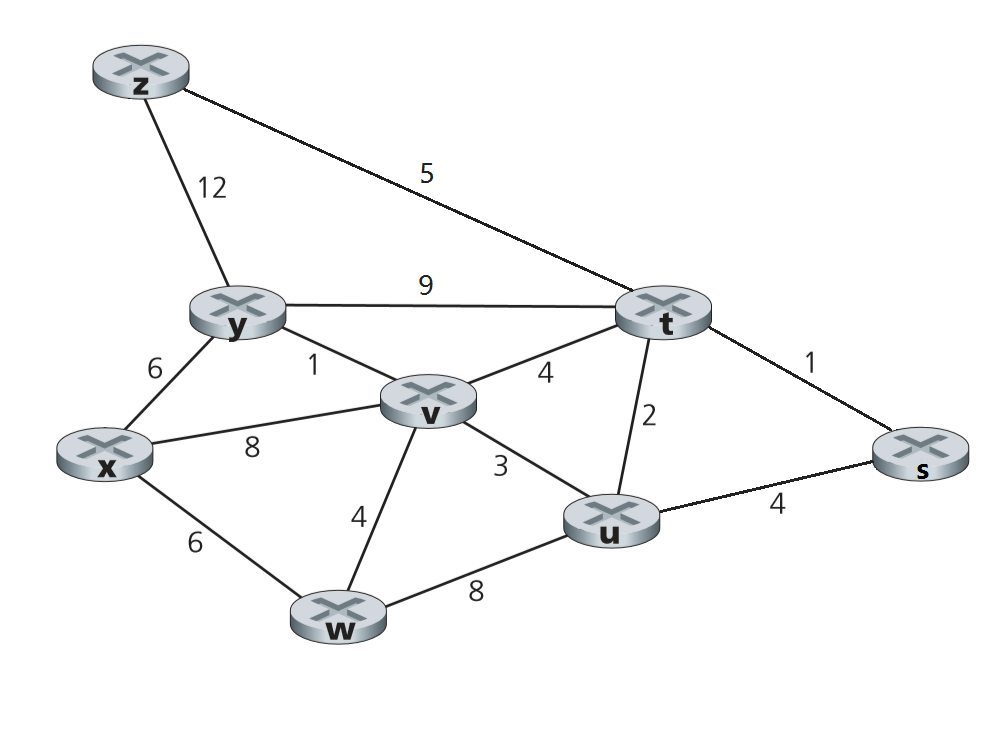
\includegraphics[width=0.8\textwidth]{4/P22.png}
    \end{figure}
	
	\begin{table}[H]
	    \centering
	    \begin{tabular}{ccccccc}
	        \hline
	        step & N' & D(v),p(v) & D(w),p(w) & D(x),p(x) & D(y),p(y) & D(z),p(z) \\
	        \hline
	        0 & u & 2,u & 5,u & 1.u & $\infty$ & $\infty$ \\
	        1 & ux & 2,u & 4,x & & 2,x & $\infty$ \\
	        2 & uxy & 2,u & 3,y & & & 4,y \\
	        3 & uxyv & & 3,y & & 4,y \\
	        4 & uxyvw & & & & & 4,y \\
	        5 & uxyvwz & & & & & \\
	        \hline
	    \end{tabular}
	    \caption{Running the link-state algorithm on the network in Figure 4.27}
	    \label{tab:4.3}
	\end{table}

	
	\item[P.25] Consider the network fragment shown below. $x$ has only two attached neighbors, $w$ and $y$. $w$ has a minimum-cost path to destination $u$ (not shown) of 5, and $y$ has a minimum-cost path to $u$ of 6. The complete paths from $w$ and $y$ to $u$ (and between $w$ and $y$) are not shown. All link costs in the network have strictly positive integer values.
	
    \begin{figure}[H]
        \centering
        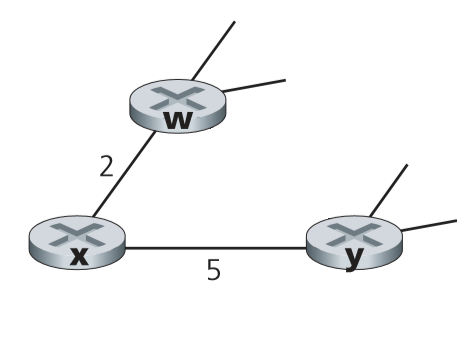
\includegraphics[width=0.3\textwidth]{4/P25.png}
    \end{figure}
	
	\begin{enumerate}[a.]
	    \item Give $x$'s distance vector for destinations $w$, $y$, and $u$.
	    \item Give a link-cost change for either $c(x, w)$ or $c(x, y)$ such that $x$ will inform its neighbors of a new minimum-cost path to $u$ as a result of executing the distance-vector algorithm.
	    \item Give a link-cost change for either $c(x, w)$ or $c(x, y)$ such that $x$ will not inform its neighbors of a new minimum-cost path to $u$ as a result of executing the distance-vector algorithm.
	\end{enumerate}
	
	\item[P.31] Consider the following network. ISP B provides national backbone service to regional ISP A. ISP C provides national backbone service to regional ISP D. Each ISP consists of one AS. B and C peer with each other in two places using BGP. Consider traffic going from A to D. B would prefer to hand that traffic over to C on the West Coast (so that C would have to absorb the cost of carrying the traffic cross-country), while C would prefer to get the traffic via its East Coast peering point with B (so that B would have carried the traffic across the country). What BGP mechanism might C use, so that B would hand over A-to-D traffic at its East Coast peering point? To answer this question, you will need to dig into the BGP specification.
	
    \begin{figure}[H]
        \centering
        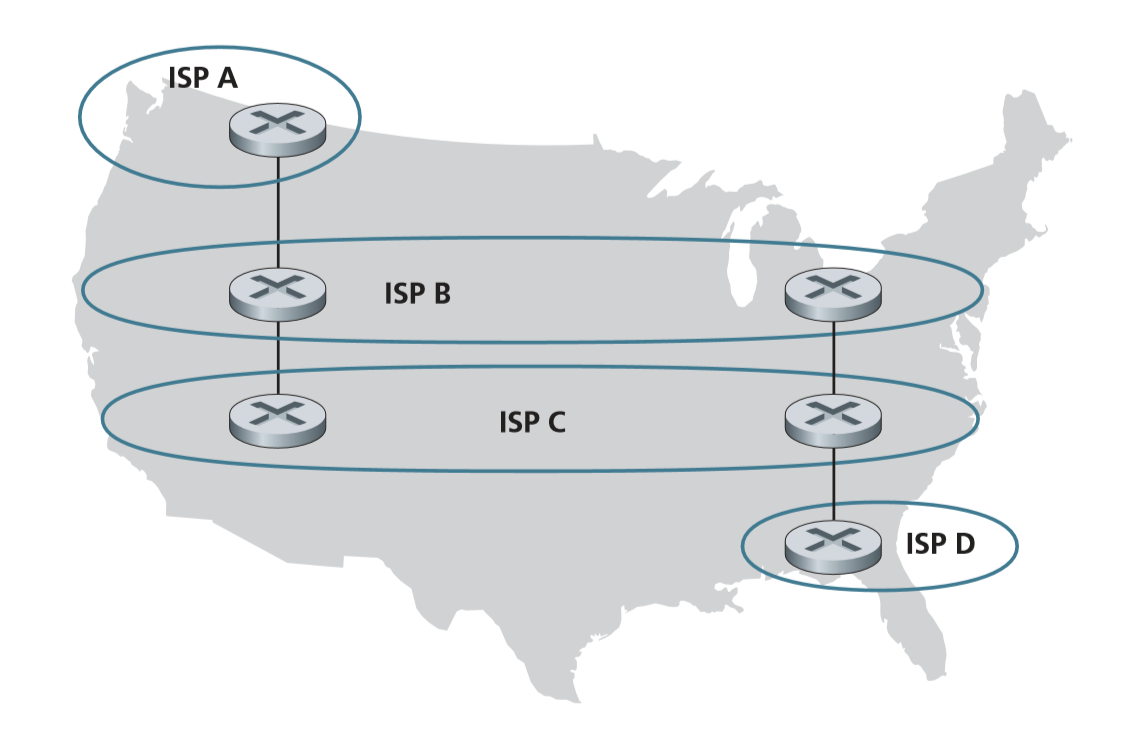
\includegraphics[width=0.8\textwidth]{4/P31.png}
    \end{figure}
	
	\item[P.35] Consider the two basic approaches identified for achieving broadcast, unicast emulation and network-layer (i.e., router-assisted) broadcast, and suppose spanning-tree broadcast is used to achieve network-layer broadcast. Consider a single sender and 64 receivers. Suppose the sender is connected to the receivers by a binary tree of routers. What is the cost of sending a broadcast packet, in the cases of unicast emulation and network-layer broadcast, for this topology? Here, each time a packet (or copy of a packet) is sent over a single link, it incurs a unit of cost. What topology for interconnecting the sender, receivers, and routers will bring the cost of unicast emulation and true network-layer broadcast as far apart as possible? You can choose as many routers as you'd like.
\end{enumerate}